\section{Particle analysis}
\label{sec:particle}

In this section, we analyze the behavior of a single particle in a swarm.
In a single stagnation, the global best is unchanged.
Thus we can have the global best as the constant.
We are interested with 
\begin{itemize}
\item whether the particle converges to the global best;
\item and the probability that the particle find a new global best.
\end{itemize}

In order to understand how the particle converges to the global best, we let $ x^{G} $ be the reference position and get Equation \eqref{eq:rel_gb}.

\begin{equation}
\label{eq:rel_gb}
\begin{aligned}
\begin{bmatrix}
v(k+1) \\
x(k+1) - x^{G}
\end{bmatrix}
 = A(k) 
\begin{bmatrix}
v(k) \\
x(k) - x^{G}
\end{bmatrix}
+ B(k) 
\begin{bmatrix}
0 \\
x^{P}(k) - x^{G}
\end{bmatrix}
\end{aligned}
\end{equation}

By Theorem \ref{coro:state_bound}, we know that $ \lVert x(k) - x^{G} \rVert $ indicates the distance to the global best, which depends on  $ \lVert x^{P}(k) - x^{G} \rVert $.

\begin{myprop}
\label{prop:particle:nonoptimal}
Whether a particle is guaranteed to reach the optimal is determined by the boundary of its movement.
\end{myprop}

\begin{figure}[tbph]
\centering
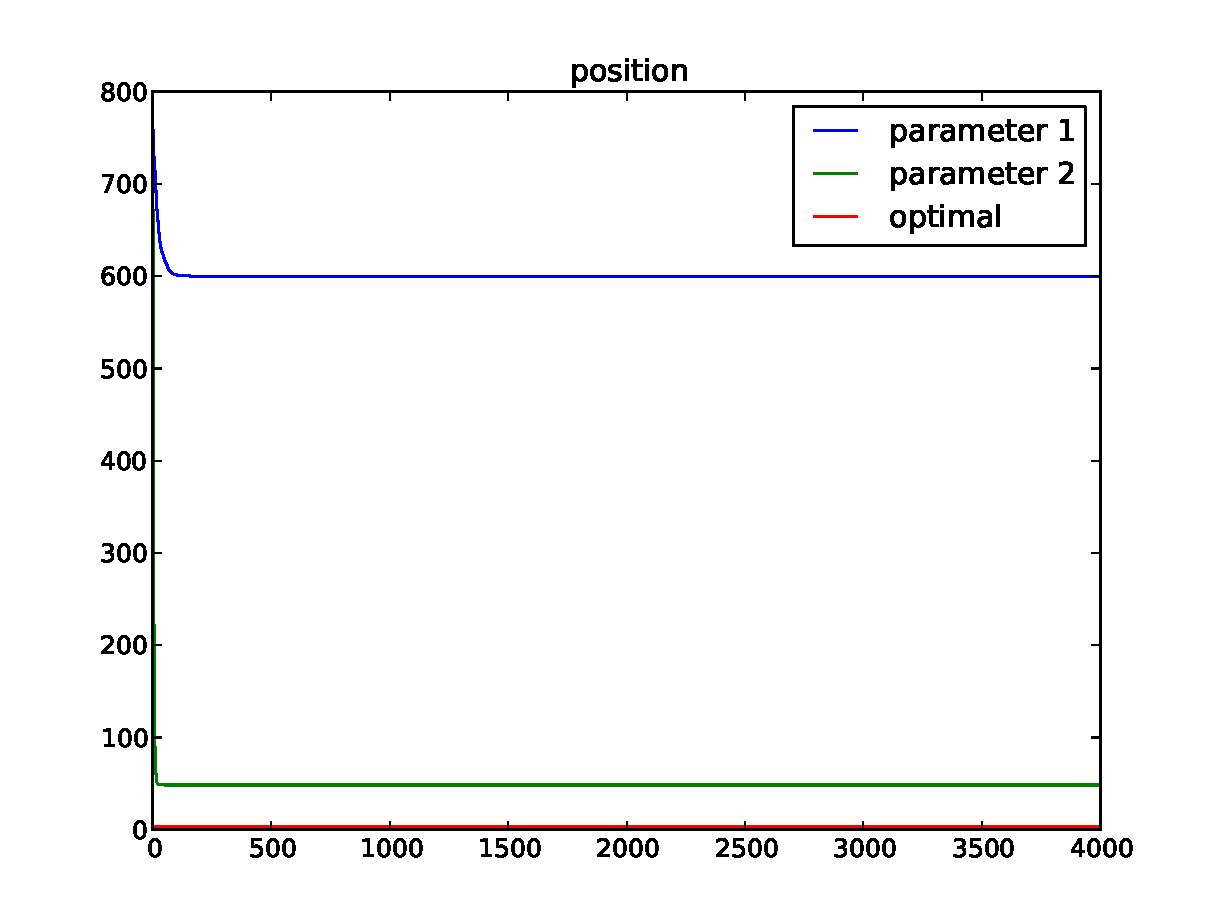
\includegraphics[width=0.7\linewidth]{./simfig/bound/bound_position}
\caption{}
\label{fig:bound_position}
\end{figure}

Figure \ref{fig:bound_position} gives an example on the boundary impacting the reach of the optimal.
Parameter 1 is $ \chi = 0.3, \phi^{P} = 0.2, \phi^{G} = 0.2 $ and parameter 2 is $ \chi = 0.72984, \phi^{P} = 2.05, \phi^{G} = 2.05 $.
As a result, parameter 1 makes a smaller movement boundary, which prevents the particle reaching the optimal.

\subsection{Unimodal fitness distribution}

A unimodal fitness distribution is most typical.
It provides a partial monotonic form and most of the cases the final convergence happens on a unimodal fitness distribution.
Any other form can usually be viewed as a combination of unimodalities as well.

When the global best is already the optimal solution, there is no chance for the particle to find a better solution and trigger a new global best.
The particle should gradually converge to the global best if the position update component is input-to-state stable, as in Lemma \ref{lem:singleHill:particle:converge}.

\begin{mylem}
\label{lem:singleHill:particle:converge}
In a unimodal case, when $ x^{G} = x^{*} $, the particle will converge to $ x^{G} $ if the update component of the particle is input-to-state stable.
\begin{proof}
When $ x^{G} = x^{*} $, the input update component is also input-to-state stable.
The serial connection of two ISS components still reserves input-to-state stability.
As the input is zero by $ \lVert x^{G} - x^{*} \rVert = 0 $, $ x(k) - x^{*} $ will converge to zero.
\end{proof}
\end{mylem}

When the global best is not yet the optimal solution, the convergence of the particle cannot be guaranteed.
If the particle accidentally reaches into a region that the fitness is better than the current global best, a new global best is found.
The particle might either runs stochastically in a region that the fitness is worse than both the personal best and the global best.
If the particle at least gets into a position that is better than the current personal best, the personal best will be updated. 
We notice that the particle should never stop at the current global best $ x^{G} $, which is stated in Lemma \ref{lem:singleHill:particle:nonstop}.

\begin{mylem}
\label{lem:singleHill:particle:nonstop}
In a unimodal case, if $ x^{G} \not = x^{*} $, a particle will never stop at $ x^{G} $. 
\footnote{The precision cut-off in implementation is ignored.}
\begin{proof}
Consider the velocity $ v(k+1) $ consists of two parts, inertia $ \chi v(k) $ and attractive force $ \chi \phi^{P} (x^{P}(k) - x(k) ) + \chi \phi^{G} ( x^{G} - x(k) ) $.
While the particle moves into $ x^{G} $, the attractive force becomes zero but the inertia still exists, due to the velocity moves the particle into this current position.
\end{proof} 
\end{mylem}

By Lemma \ref{lem:singleHill:particle:nonstop}, we can prove that the particle will finally get to a position that is at least better than the current global best if given enough run time.
We have Theorem \ref{thm:singleHill:particle:better}.

\begin{mythm}
\label{thm:singleHill:particle:better}
In a unimodal case, the particle will almost surly find a $ \hat{x^{*}} $ that $ f(\hat{x^{*}}) > f(x^{G}) $ if $ f( x^{G} ) < f( x^{*}) $.
\begin{proof}
Because the particle cannot stop at $ x(k) = x^{G} = x^{P} $.
It will finally arrives into a region that $ f(x) > f(x^{G}) $.

As in Figure \ref{fig:categorize_regions}, the solution space will be divided into three types of regions by the global best and the personal best.
\begin{itemize}
\item $ f(x) > f(x^G) $
Once a particle gets into this region, it updates both global best and personal best. 
It becomes a leader of the swarm.
\item $ f(x^{G}) > f(x) > f(x^{P}) $
Once a particle gets into this region, it updates only the personal best.
The solution space is then re-divided.
\item $ f(x) < f(x^{P}) $
When a particle is in this region, it only moves as a random walk.
\end{itemize}

\begin{figure}
\centering
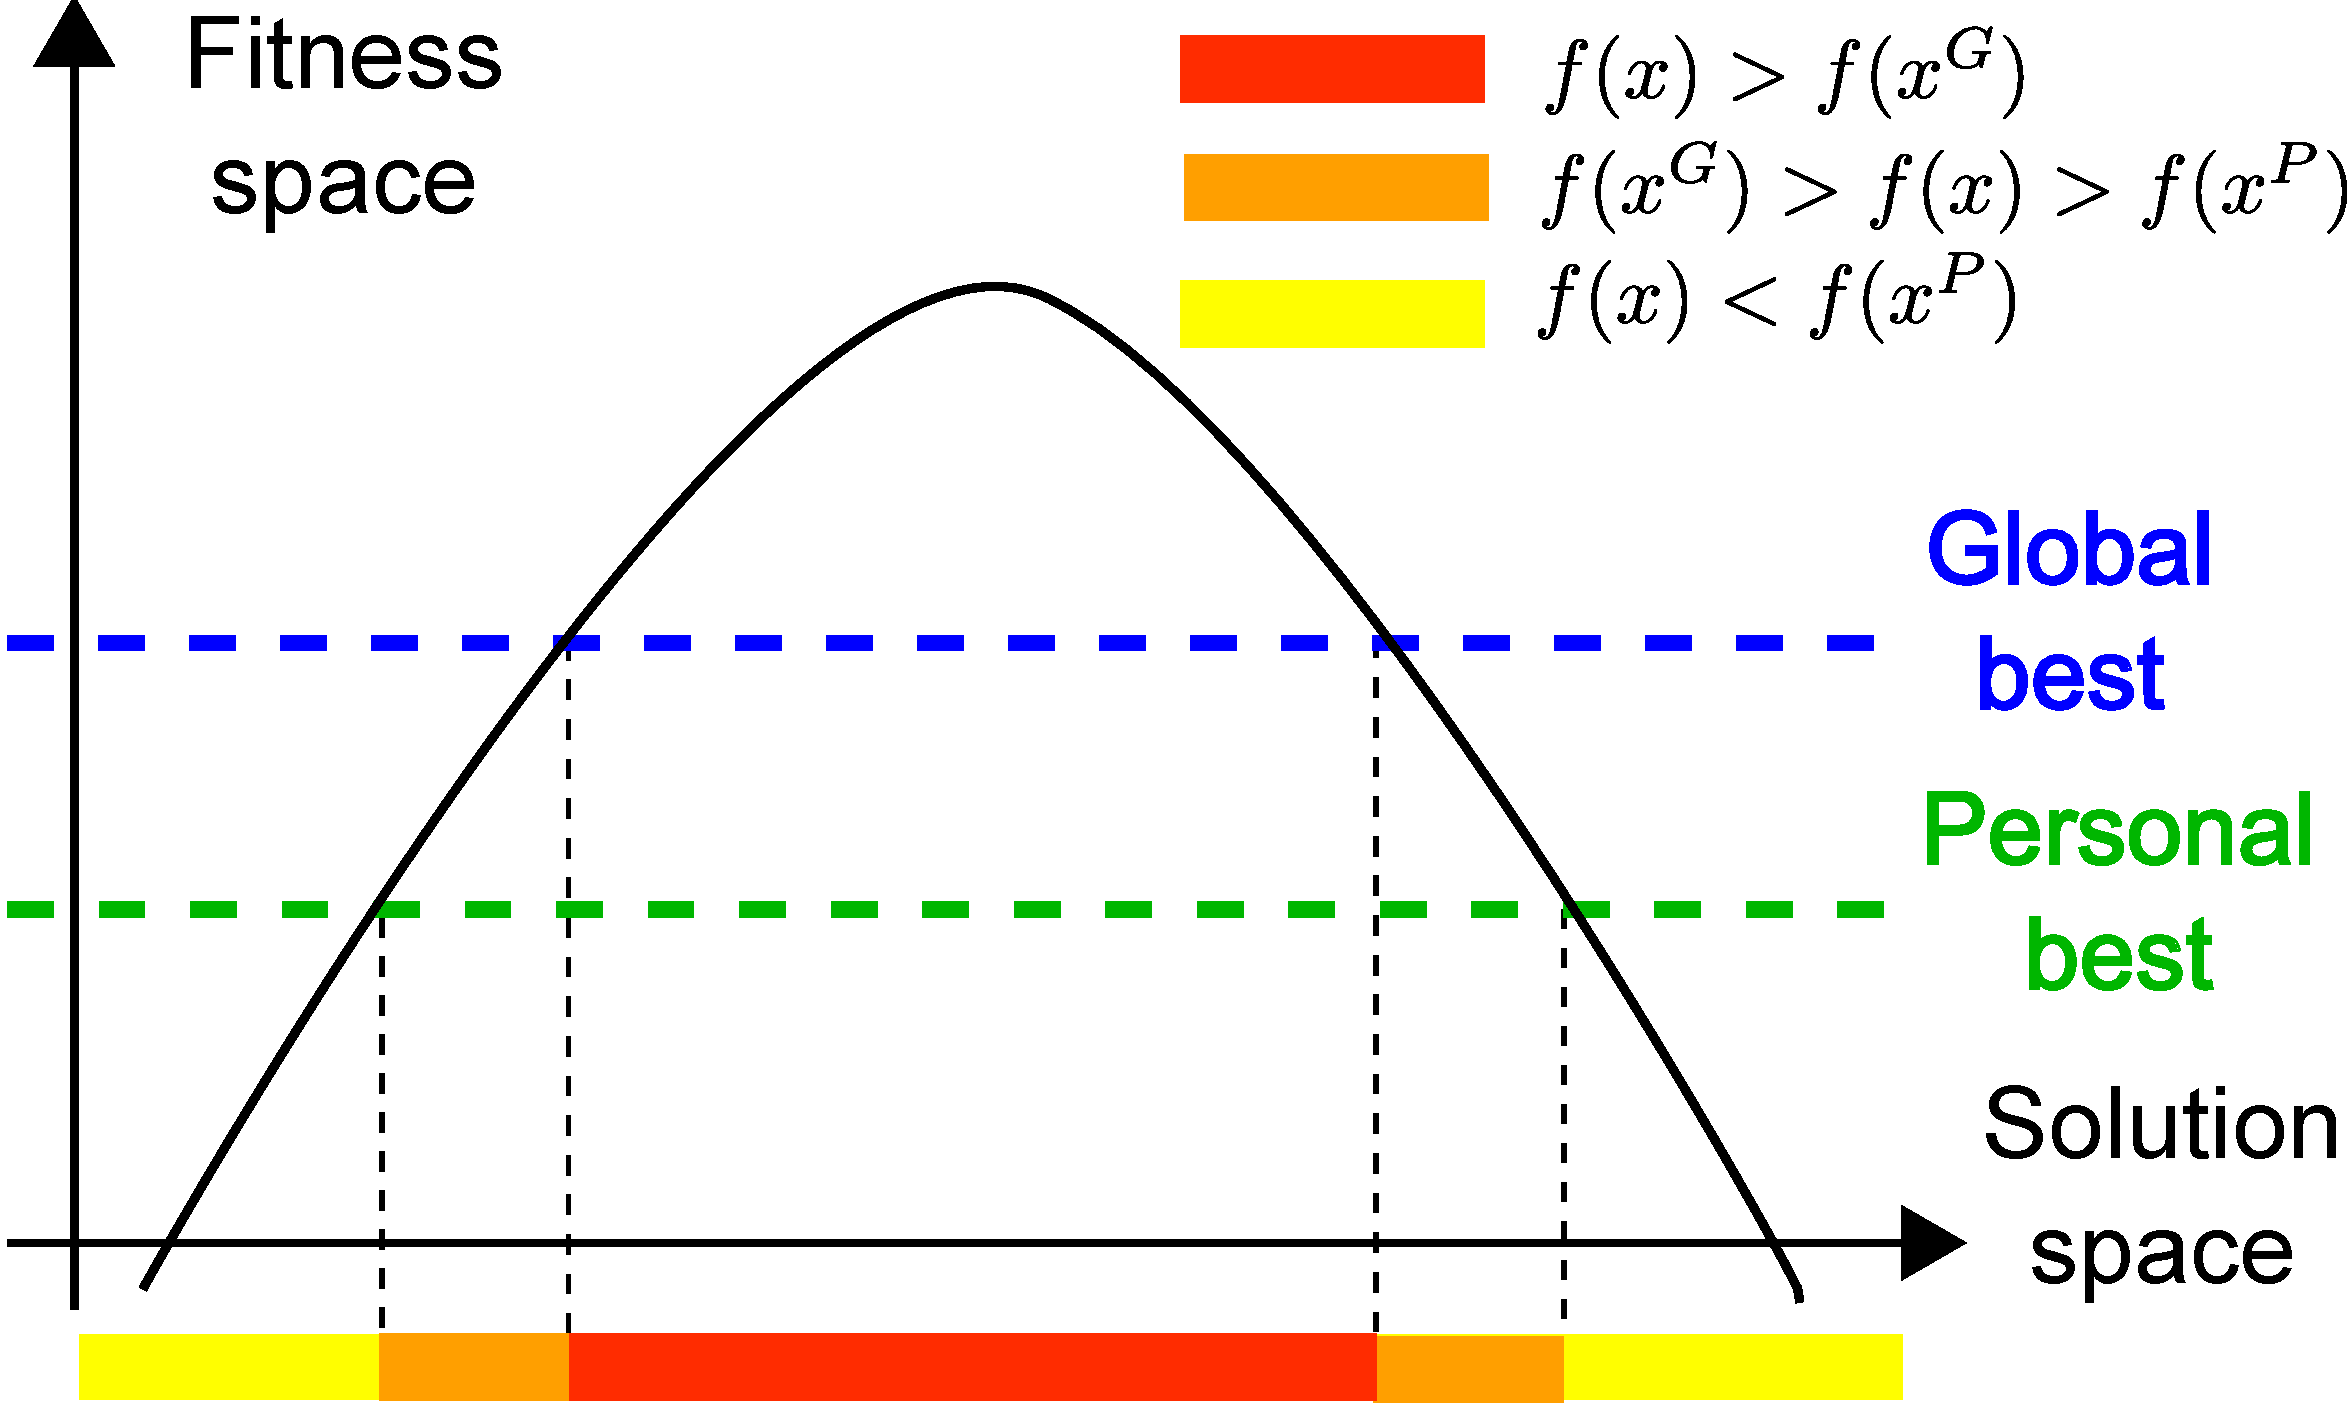
\includegraphics[width=0.7\linewidth]{./fig/categorize_regions}
\caption{How global best and personal best divide the solution space.}
\label{fig:categorize_regions}
\end{figure}

The result of the movement of a particle is determined by which region of the solution space it moves in.
The states of the particle can be defined as
\begin{itemize}
\item \textbf{A} [$ f(x) \leq f(x^{P}) \leq f(x^{G}) $]
\item \textbf{B} [$ f(x) = f(x^{P}) \leq f(x^{G}) $] 
\item \textbf{C} [$ f(x) = f(x^{P}) \leq f(x^{G}) \land v > 0 $]
\item \textbf{D} [$ f(x) = f(x^{P}) \leq f(x^{G}) \land v = 0 $]
\item \textbf{E} [$ f(x) > f(x^{P}) = f(x^{G}) $]
\end{itemize}

The Figure \ref{fig:fsm} shows the state transitions.
When the particle is in state A, it is in random walk with attractions to the global best and personal best.
In state B, it means that the particle find a better personal best.
In state C, the particles moves into the current global best, but the velocity is not zero yet.
The only chance that the particle cannot find a better global best happens when it gets into state D.

\begin{figure}[tbph]
\centering
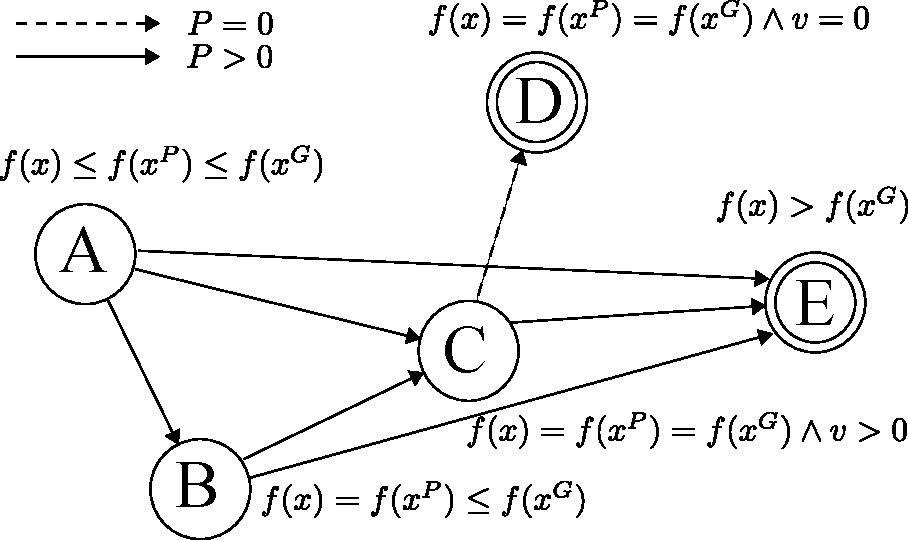
\includegraphics[width=0.7\linewidth]{./fig/fsm}
\caption{The state transition of the movement of the particle.}
\label{fig:fsm}
\end{figure}

\end{proof}
\end{mythm}

\subsubsection{Exploitation}

The design of the position component of a particle imports the exploitation of the optimal search.
When input-to-state stability is guaranteed, a single particle shows the convergence in a unimodal case.
The personal best and the global best attracts the particle moving toward themselves~\cite{Schmitt:2013:PSO:2463372.2463563}.

The input-to-state stability guarantees that the particle could utilize the current information as the heuristic.


\subsection{Multi-model fitness distribution}

When there are multiple modalities in the range that the particle moves, it is not easy to figure out a pattern of the behaviors that the particles share.
More factors of the fitness distribution can impact the optimal search process.
When the movement of the particle is bounded, there can be cases that the particle cannot reach the region that contains a better solution.
%[TODO: Give an example that the particle will wander between the personal best and the global best]

The exploration range is determined by the boundary of a particle's movement.

\begin{mylem}
\label{lem:particle:bound_mov}
The bound of a particle's movement is 
\begin{equation}
\lVert x(k) - x^{*} \rVert < \delta ( \max ( \lVert x^{G} - x^{*} \rVert , \lVert x^{P}(k) - x^{*}  \rVert ) ),
\end{equation}
in which $ \delta () $ is a boundary function. 
\end{mylem}

Lemma \ref{lem:particle:bound_mov} shows that the boundary of a particle's movement is determined by where the global best $ x^{G} $ and the personal best $ x^{P}(k) $ locate at.

[TODO] Add how the new global best might be found or not be found.

As we are interested with the probability that the particle gets into a position that is better than the current global best, we hope the distance from this position to the optimal is closer than that from the global best to the optimal.

In order to measure how likely the particle can moves to a position that $ f(x) > f(x^{G}) $, we can measure the probability of that $ \lVert x(k) - x^{*} \rVert < \lVert x^{G} - x^{*} \rVert $ indirectly.

\begin{mycoro}
\label{lem:nonsingleHill:particle:prob}
\begin{equation}
\begin{aligned}
& P( \lVert x(k) - x^{*} \rVert < \lVert x^{G} - x^{*} \rVert ) \\
& > 1 - \frac{ \delta ( \max ( \lVert x^{G} - x^{*} \rVert , \lVert x^{P}(k) - x^{*}  \rVert ) ) }{ \lVert x^{G} - x^{*} \rVert },
\end{aligned}
\end{equation}
in which $ \delta () $ is a boundary function.
\begin{proof}
By Markov's inequality, we have
\begin{equation}
P( \lVert x(k) - x^{*} \rVert \geq \lVert x^{G} - x^{*} \rVert ) \leq \frac{ E( \lVert x(k) - x^{*} \rVert ) }{ \lVert x^{G} - x^{*} \rVert }.
\end{equation} 
By the boundary, we have
\begin{equation}
E( \lVert x(k) - x^{*} \rVert ) \leq \delta ( \max ( \lVert x^{G} - x^{*} \rVert , \lVert x^{P}(k) - x^{*}  \rVert ) ),
\end{equation}
in which $ \delta () $ is the boundary function.
\begin{equation}
\begin{aligned}
& P( \lVert x(k) - x^{*} \rVert < \lVert x^{G} - x^{*} \rVert ) \\
= & 1 - P( \lVert x(k) - x^{*} \rVert \geq \lVert x^{G} - x^{*} \rVert ) \\
> & 1 - \frac{ E( \lVert x(k) - x^{*} \rVert ) }{ \lVert x^{G} - x^{*} \rVert } \\
> & 1 - \frac{ \delta ( \max ( \lVert x^{G} - x^{*} \rVert , \lVert x^{P}(k) - x^{*}  \rVert ) ) }{ \lVert x^{G} - x^{*} \rVert }.
\end{aligned}
\end{equation}
\end{proof}
\end{mycoro}

\subsubsection{Exploration}


